\authoredsubsection{Sprint 3}{Marco}{Marco-Fabian Schröder}\label{sec:sprint3}

Sprint 3 ran from 26 May to 09 June 2026, with the review and retrospective held on 09 June. Sprint 2 had established the main pipeline components as separate, independently functional modules, so the objective of this sprint was to shift from further improving individual capability in the first half toward preparing these modules for integration into a single executable loop in the second half of the sprint. Two open questions shaped the work: how to optimize the router's two stages separately, and how to redesign the judge to reduce the systematic biases identified in its first evaluation. In addition, Interhyp had encouraged the team during the Sprint 2 review to prioritize measurable evaluation results over further scope expansion, which set the tone for the sprint. Marco Schröder took over the role of the Scrum Master for this sprint.

\subsubsection{Sprint Goals}\label{sec:sprint3-goals}

The team committed to creating a new evaluation dataset with more challenging routing cases and to validating and improving the judge until its evaluations are more accurate than the router's decisions. For the router, the goal was to find suitable per-agent thresholds for Stage 1 and to build a dashboard that visualizes the effect of different threshold settings on accuracy and latency. The sprint further included a proof of concept of the optimizer with the DSPy optimization framework and the preparation of the end-to-end integration of router, judge, and optimizer on a data format level toward a first optimization run producing an improved router prompt. The team also prepared the mid-term presentation within this sprint.

\subsubsection{Sprint Planning}\label{sec:sprint3-planning}

The team decided that the increasing maturity of the individual components justified restructuring the backlog into component-oriented epics for the router, judge, optimizer, and documentation work. Backlog items were deliberately kept small, with a maximum estimate of three story points per item, to promote fast intermediate deliveries and early discussions on the integration. The sprint contained 25 story points in total, consistent with the velocity of the previous sprints. The established stand-up cadence was retained, with the Sunday stand-up moved to the morning and extended to one hour to give the team more preparation time ahead of the mid-term presentation.

\Cref{fig:sprint3-backlog} shows the user stories that were included in the sprint backlog for Sprint 3. The only item which had a story point estimate of more than three story points was the preparation of the slides for the mid-term presentation with five story points, but this was equally split across the team through subtasks with one story point per team member.

\begin{figure}
\centering
\pandocbounded{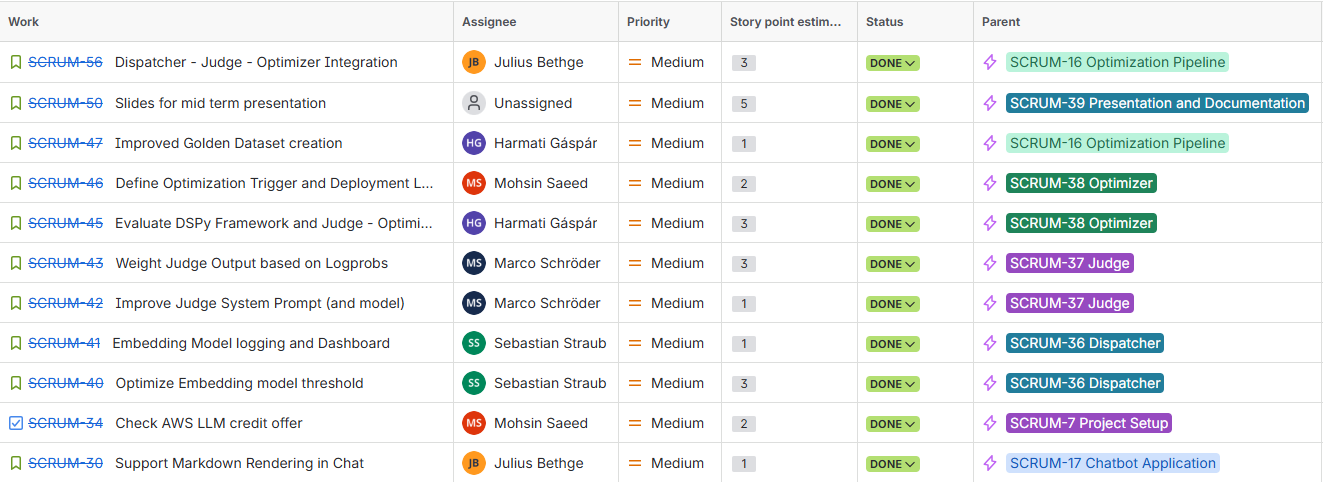
\includegraphics[keepaspectratio]{assets/sprints/sprint3-backlog.png}}
\caption{Sprint 3 Backlog in Jira with owners and completion status.}
\label{fig:sprint3-backlog}
\end{figure}


\subsubsection{Implementation and Execution}\label{sec:sprint3-execution}

The largest block of work concerned the router's first stage. Its reference store was redesigned from formal agent descriptions to sets of example queries per agent, since embedding models perform more reliably on semantically symmetric inputs such as query-to-query comparisons than on asymmetric pairs of short queries that are compared to long descriptions \autocite{gao2023hyde}. The embedding model itself was upgraded from BAAI/bge-small-en-v1.5 to intfloat/multilingual-e5-large, guided by the Massive Text Embedding Benchmark \autocite{muennighoff2023mteb}, while keeping Stage 1 latency at approximately 100 ms. Even higher performing models were not selected due to external API dependencies that would have introduced per-query cost. The thresholding logic was revised from a single global threshold to per-agent margin thresholds between the top two candidates, calibrated on 1,000 queries from the golden dataset. In addition, the full similarity vector of all eight agents was logged for every Stage 1 decision. A dashboard visualizes the effect of different threshold settings on routing accuracy and time saved (\cref{fig:sprint3-thresholds}). Following a data-leak warning from the Product Owner Julian, the team decided that new Stage 1 example queries should never originate from the golden dataset as this would lead to artificially perfect results, and a separate dataset of 250 ambiguous queries was created for this purpose.

\begin{figure}
\centering
\pandocbounded{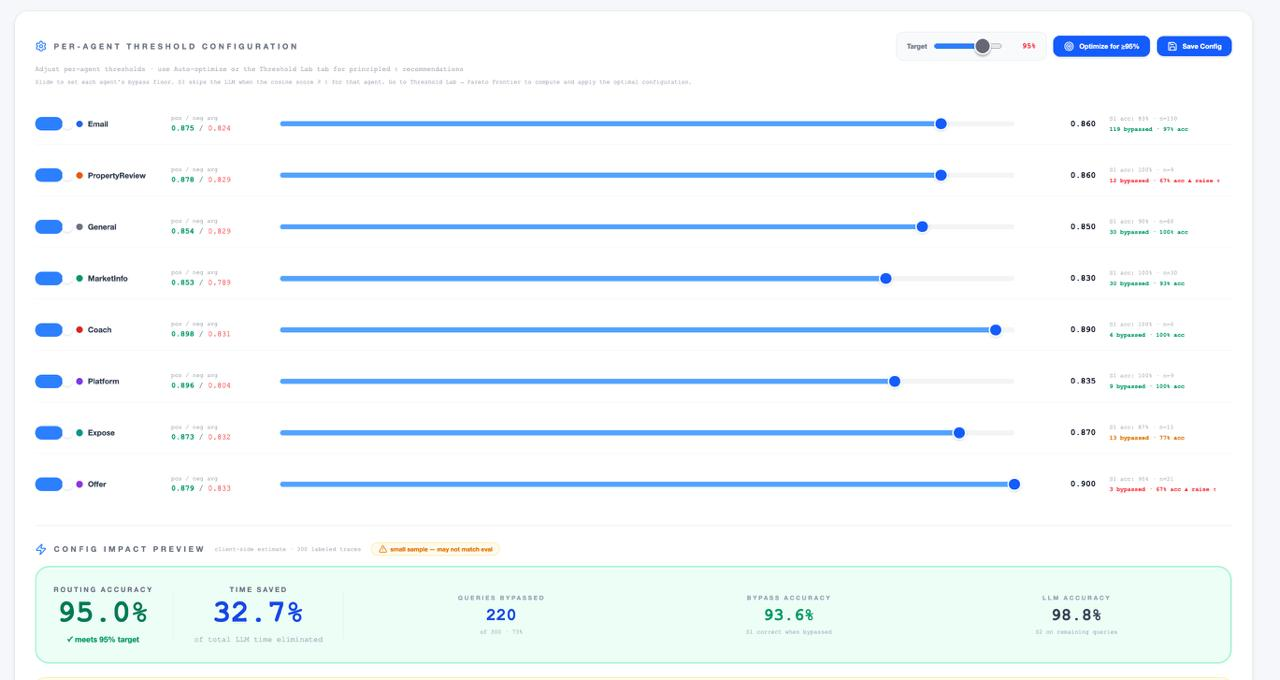
\includegraphics[keepaspectratio]{assets/sprints/sprint3-threshold-dashboard.png}}
\caption{Dashboard for exploring per-agent margin thresholds in Stage 1.}
\label{fig:sprint3-thresholds}
\end{figure}


The second focus was the redesign of the judge. Its first evaluation, run with a generic comparison prompt on Gemma 4 31B, reached only 51\% agreement with the ground truth on the 100 most uncertain queries, and the root cause analysis identified a systematic style bias toward the highly formatted responses of the MarketInfoAgent. The prompt was redesigned around routing-specific evaluation rubrics that are applied in a sequential, form-filling scheme. After the AWS Bedrock access was validated and ensured in this sprint, the judge model was additionally migrated to Claude Sonnet 4.6 under a hybrid architecture in which the router continues to run locally while compute-intensive components use cloud models. This raised judge accuracy to 98\% on the training dataset and 99\% on the evaluation dataset. An exploration of token log-probabilities as a judge confidence signal was closed without result. The evaluated model commits to its decision internally before generating the output, so the log-probabilities degenerate to complete certainty values of 100\% for the winning agent that carry no usable information.

In parallel, the team evaluated the DSPy framework \autocite{khattab2024dspy} as a possible replacement for the self-built OPRO optimizer. The proof of concept used its MIPROv2 optimizer and a deployment guard that rolls back any new prompt below a two-percentage-point improvement. The optimized prompt scored identically to the baseline, which exposed a conceptual issue rather than a tuning problem: the evaluation ran through both Stages of the router, so Stage 1 resolved nearly all validation queries before the optimized Stage 2 prompt was ever exercised. This led to the result that not enough queries were evaluated to produce statistically relevant insights. The knowledge that optimization runs must target Stage 2 directly was carried into the next sprint, together with the pending decision between DSPy and the self-built optimizer. The story for the DSPy optimizer was still closed as a PoC integrating the framework was set up.

Finally, the sprint laid the groundwork for integration. The team mapped all module interfaces in an in-person whiteboard session and connected the pipeline through three links: the judge runs as an asynchronous background process on every router request, its corrections are written to an isolated correction file that mirrors the Stage 1 example format without contaminating it, and the optimizer is triggered manually using the judge's output data format so that generated prompts can be reviewed before deployment. The proposal by Julius to replace this direct coupling with a dedicated orchestration layer to ensure the integration of the pipeline into the Chatbot application became the main priority for Sprint 4.

\subsubsection{Sprint Review}\label{sec:sprint3-review}

The review took place at the Interhyp office on 09 June 2026 and was extended to two hours, with additional colleagues of Julian and Rainer joining the second half of the meeting so that the team could practice the mid-term presentation and gather broader technical feedback. Julian and Rainer appreciated the threshold dashboard for making the tradeoff between routing accuracy and time saved immediately visible and were interested in exploring an optimization approach for the per-agent thresholds themselves in the future. They emphasized that the pipeline stands or falls with the judge and cautioned that, as router accuracy improves, a stagnating judge could begin to drag accuracy down rather than lift it. The team agreed that in a production setting it would be required to periodically re-evaluate the judge on newly labeled queries. The audience additionally proposed crowdsourcing ambiguous router cases by letting chatbot users choose between the two best agent responses, which would distribute annotation effort across all users and offer a possibility in the production system to evaluate the judge's performance.

All 25 story points were completed. The burndown chart (\cref{fig:sprint3-burndown}) shows three conspicuous patterns. It starts from a zero baseline because the sprint was technically started immediately after the old sprint was closed in Jira, but the sprint planning session still had to be conducted. As during the sprint planning session all items were moved to the sprint backlog, there is an increase of 25 story points one day after the sprint started. Second, there is a slight increase and immediate decrease in story points one day after the sprint planning happened as the DSPy optimizer PoC turned out to be more complex than expected, but at the same time the creation of additional ground truth queries required less effort than estimated as the same procedure had already been performed in the previous sprint. Also, most items were closed in the second half, which reflects the dependency of the integration work on the completion of the individual module tickets.

\begin{figure}
\centering
\pandocbounded{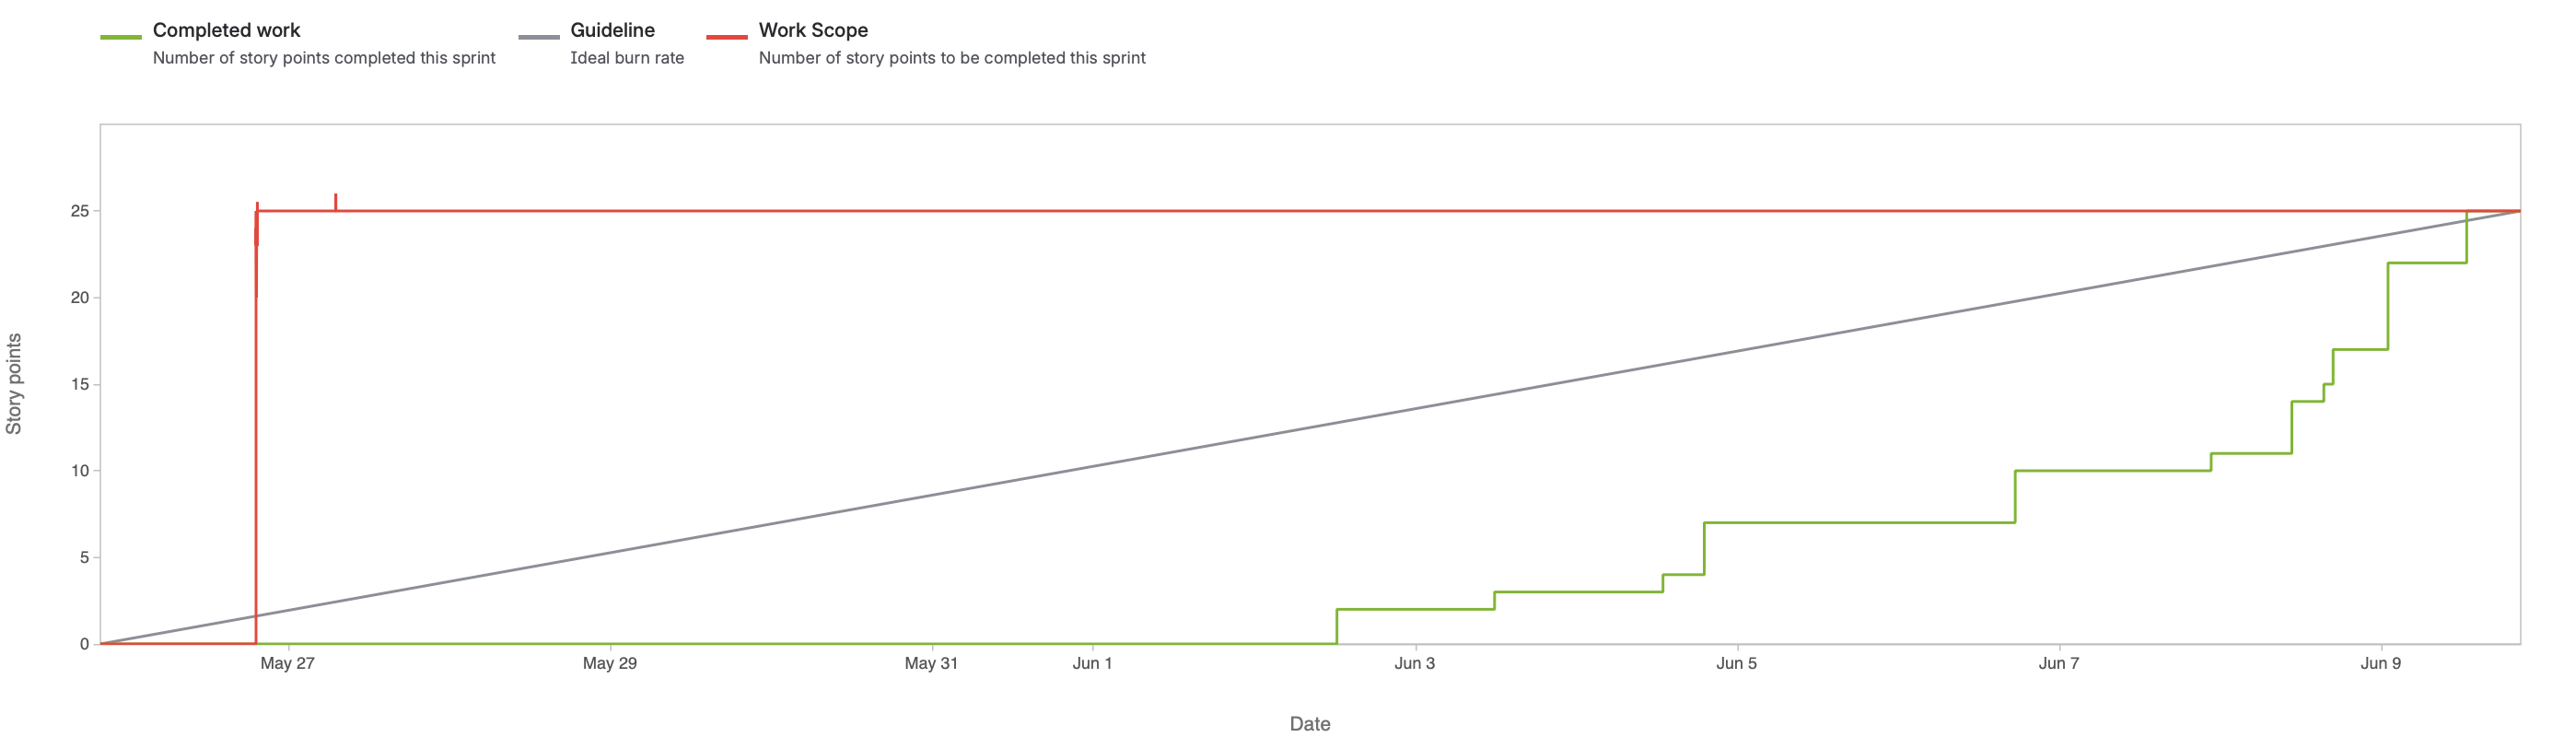
\includegraphics[keepaspectratio]{assets/sprints/sprint3-burndown.png}}
\caption{Sprint 3 burndown chart.}
\label{fig:sprint3-burndown}
\end{figure}


\subsubsection{Sprint Retrospective}\label{sec:sprint3-retrospective}

The sprint retrospective was held on 09 June 2026, directly after the sprint review meeting. In the opening exercise, team members reviewed the sprint in the style of a product review on Amazon with a star rating, which converged on three to four out of five stars. The sprint felt productive but stressful and at times messy, mainly because preparing the integration revealed more architectural complexity than the estimates had anticipated. A lot of discussions were happening based on ad-hoc and late-night calls to clarify misunderstandings about the individual module outputs. The team concluded that user stories need to be discussed in more detail during planning to reach realistic estimates (\cref{fig:sprint3-retrospective}).

\begin{figure}
\centering
\pandocbounded{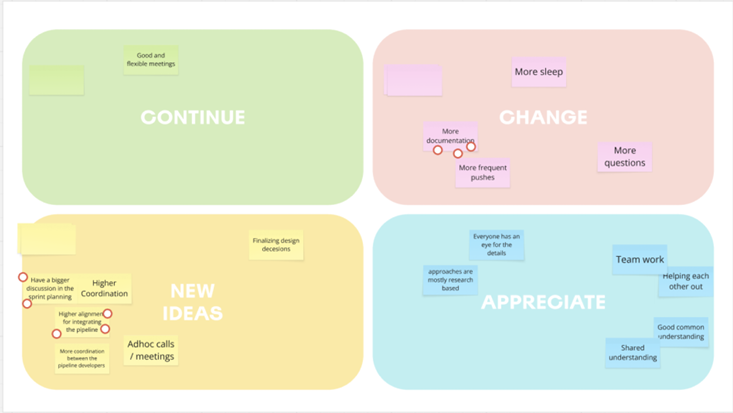
\includegraphics[keepaspectratio]{assets/sprints/sprint3-retrospective.png}}
\caption{Sprint 3 retrospective feedback collection in Miro.}
\label{fig:sprint3-retrospective}
\end{figure}


Two action items were derived for the following sprint: a dedicated meeting on the functional integration of the modules directly after the mid-term presentation, and an increase to four meetings per week, including a Monday evening slot to clarify open questions ahead of the weekly in-person session (\cref{fig:sprint3-actions}).

\begin{figure}
\centering
\pandocbounded{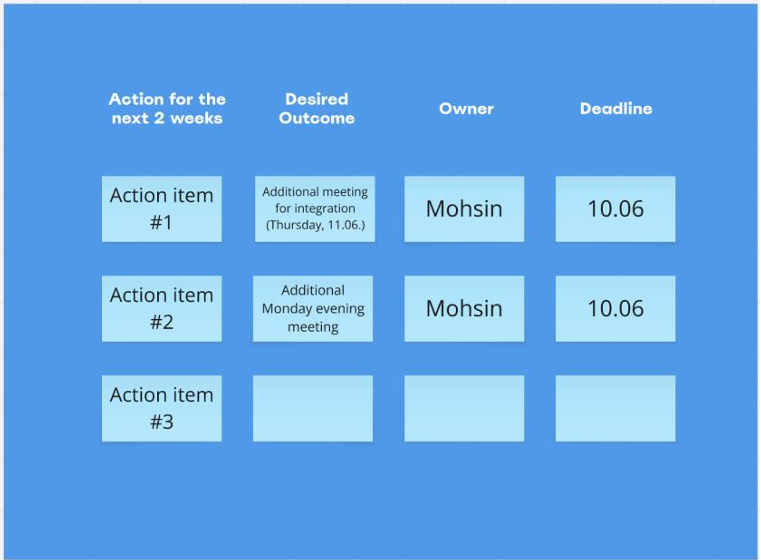
\includegraphics[keepaspectratio]{assets/sprints/sprint3-action-items.png}}
\caption{Action items for Sprint 4.}
\label{fig:sprint3-actions}
\end{figure}
